\documentclass{article}
\usepackage[margin=1in]{geometry}
\usepackage[outdir=./]{epstopdf}  					% Avoids errors when input figures
\usepackage[labelsep=period,labelfont=bf]{caption}
%\usepackage{subcaption}
\usepackage{graphicx}
%\graphicspath{{../Figures/LPs/LagDep-FX/Target/EM/}{../Figures/LPs/LagDep-FX/Path/EM/}{../Figures/LPs/LagDep-FX/LSAP/EM/}}

\begin{document}
	\begin{figure}[tbph]
		\caption{Response of the EM Yield Curve to a Forward Guidance Surprise: 2000-2019} \label{fig:LPEMpathWh}
		\begin{center}
			\begin{minipage}{\linewidth}
				\begin{center}
					\begin{subfigure}[t]{\linewidth}
						\includegraphics[trim={0cm 0cm 0cm 0cm},clip,height=0.35\textheight,width=\linewidth]{../Figures/LPs/LagDep-FX/Path/EM/PathEMnomyptpphi120m.eps} \\
						\vspace{-0.35cm}
						\caption{10-Year Yield} \label{subfig:LPEM10YpathWh}
					\end{subfigure}
					
					\vspace{0.5cm}
					
					\begin{subfigure}[t]{\linewidth}
						\includegraphics[trim={0cm 0cm 0cm 0cm},clip,height=0.35\textheight,width=\linewidth]{../Figures/LPs/LagDep-FX/Path/EM/PathEMnomyptpphi24m.eps} \\
						\vspace{-0.35cm}
						\caption{2-Year Yield} \label{subfig:LPEM2YpathWh}
					\end{subfigure}
				\end{center}
				\fignotes{This figure shows the response following \cite{Jorda:2005} of the 10- and 2-year emerging market (EM) nominal yields and their components to a forward guidance surprise. Nominal yields are decomposed into an expected future short-term interest rate, a term premium and a credit risk compensation, see section \ref{sec:Decomposition} for details. Forward guidance surprises are identified using high-frequency data around Fed's monetary policy announcements, see section \ref{sec:USMPS} for details. The 90\% confidence bands are based on Driscoll--Kraay standard errors.}
			\end{minipage}
		\end{center}
	\end{figure}
\end{document}
% trim = {<left> <lower> <right> <upper>}